% learn about REVTeX at https://journals.aps.org/revtex
% useful references:
%   https://cdn.journals.aps.org/files/revtex/summary4-1.pdf
%   ftp://ftp.dante.de/tex-archive/info/latex-refsheet/LaTeX_RefSheet.pdf
%   http://www-groups.mcs.st-andrews.ac.uk/~alanc/pub/c_tikzref/c_tikzref.pdf
\documentclass[
%draft,
aps,prd,
preprint,
onecolumn,
12pt,
amsmath, amssymb,
secnumarabic,
]{revtex4-1}

\usepackage[utf8]{inputenc}
\usepackage{minted}
\usepackage[dvipsnames]{xcolor}
\usepackage{standalone}
\usepackage{multirow}
\usepackage{longtable}
\usepackage{siunitx}
\usepackage{graphicx}
\usepackage[italicdiff]{physics}
\usepackage{tikz}

\usetikzlibrary{decorations.markings}
\usetikzlibrary{calc}
\graphicspath{{../png/}}
\usemintedstyle{vs}
\setminted[python]{mathescape=true,python3=true}

\newcommand{\comment}[1]{}
\newcommand{\python}[1]{\textcolor{BrickRed}{\texttt{#1}}}

\begin{document}

\title{Gravispy: Gravitational Simulations in Open Source Software}
\homepage{https://github.com/cjayross/gravispy}
\author{Spence Norwood}
\author{Kellen O'Keefe}
\author{Calvin Ross}
\affiliation{University of Texas at Dallas, Physics Department}
\begin{abstract}
  Lorem ipsum dolor sit amet, consectetur adipiscing elit.
  Curabitur venenatis ultricies purus, vel pellentesque tortor pellentesque vulputate.
  Sed a tincidunt felis.
  Integer ultrices, dui in maximus ultrices, leo erat aliquet diam, ut interdum sapien turpis eget lorem.
  Phasellus lectus augue, vehicula vel faucibus sed, dapibus in dolor.
  Vivamus interdum diam vitae fermentum mollis.
  Donec tortor sem, mollis ut tincidunt ut, iaculis id quam.
  In nunc lorem, mattis id hendrerit eget, accumsan vitae odio.
  Morbi ipsum massa, volutpat eget magna hendrerit, pellentesque pellentesque augue.
  Fusce a convallis massa, non mattis nisl.
  Mauris ac luctus sem.
  Aenean dui eros, blandit in nisl et, porta malesuada diam.
  Sed eget turpis eget erat vehicula condimentum.
  Donec eu tellus ultricies, luctus massa non, convallis lacus.
  Nunc fringilla porttitor sem nec luctus.
  Quisque tincidunt dui id finibus facilisis.
  Proin in consectetur risus, ut ornare ipsum.

  Phasellus gravida leo nec quam sagittis, non semper quam molestie.
  Praesent sed commodo tortor, et ultrices tellus.
  Suspendisse malesuada sed mi quis ultrices.
  Suspendisse quis purus non ligula commodo tempor sit amet eget massa.
  Vivamus nunc diam, elementum sit amet est a, aliquam ultrices purus.
  Phasellus vestibulum enim nisl, at luctus leo mattis eu. Fusce non commodo est.
\end{abstract}
\maketitle

\section{Introduction}
\documentclass{standalone}

\begin{document}


\end{document}


\section{Motivation}
\documentclass{standalone}

\begin{document}


\end{document}


\section{Methods}
\documentclass{standalone}

\begin{document}

\begin{figure*}
  \caption{\label{fig:imgbuild}
    Illustration marking intermediary steps during the image forming process.
    The new image is first created that defaults to black.
    During execution, the \emph{apply\_lens} algorithm iterates through each pixel of the newly generated image and uses the passed lensing map to determine which pixel from the input should be placed at that location.}
  \begin{tikzpicture}[>=stealth,line width=3pt]
    \tikzset{every node/.style={inner sep=0pt}}
    \def\voffset{3.75cm}
    \def\hoffset{5cm}
    \node (in) at (-\hoffset,0pt)
      {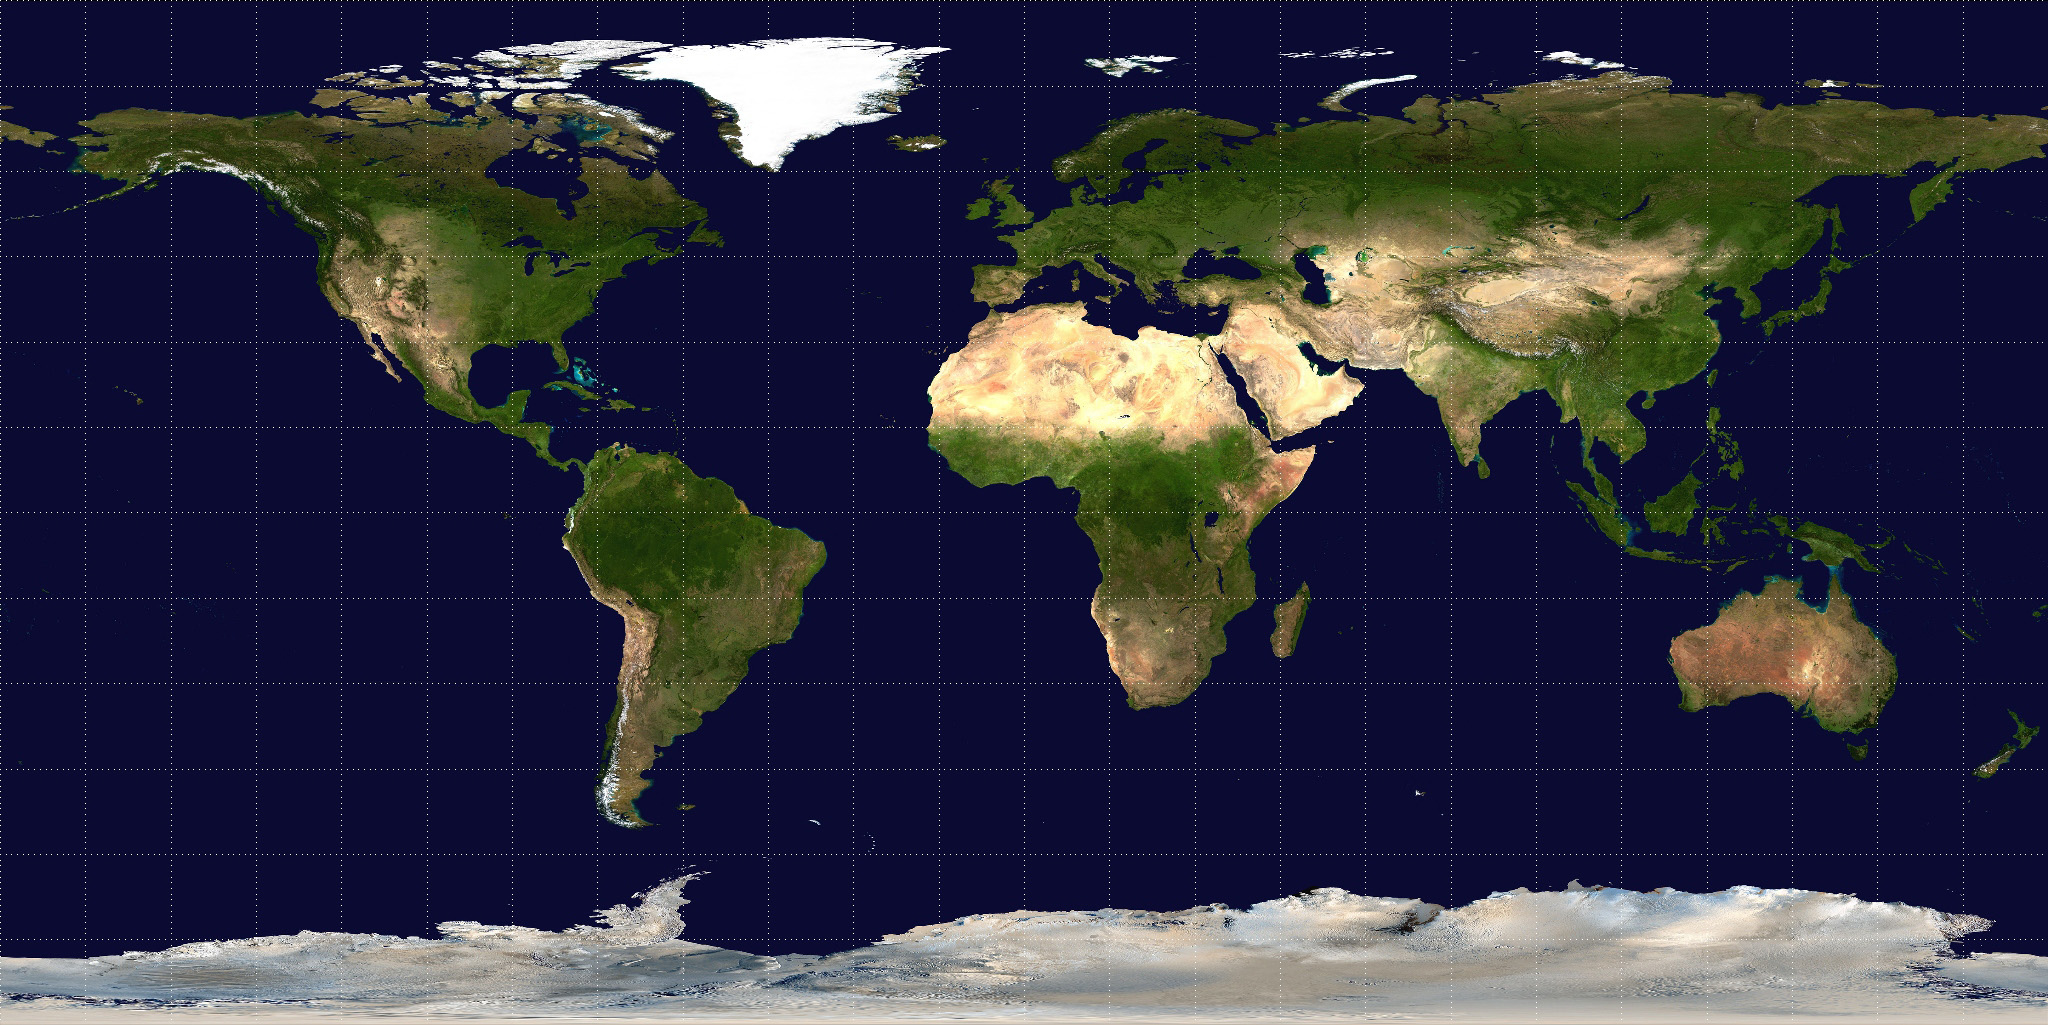
\includegraphics[width=.4\textwidth]{earth}};
    \node (out1) at (\hoffset,\voffset)
      {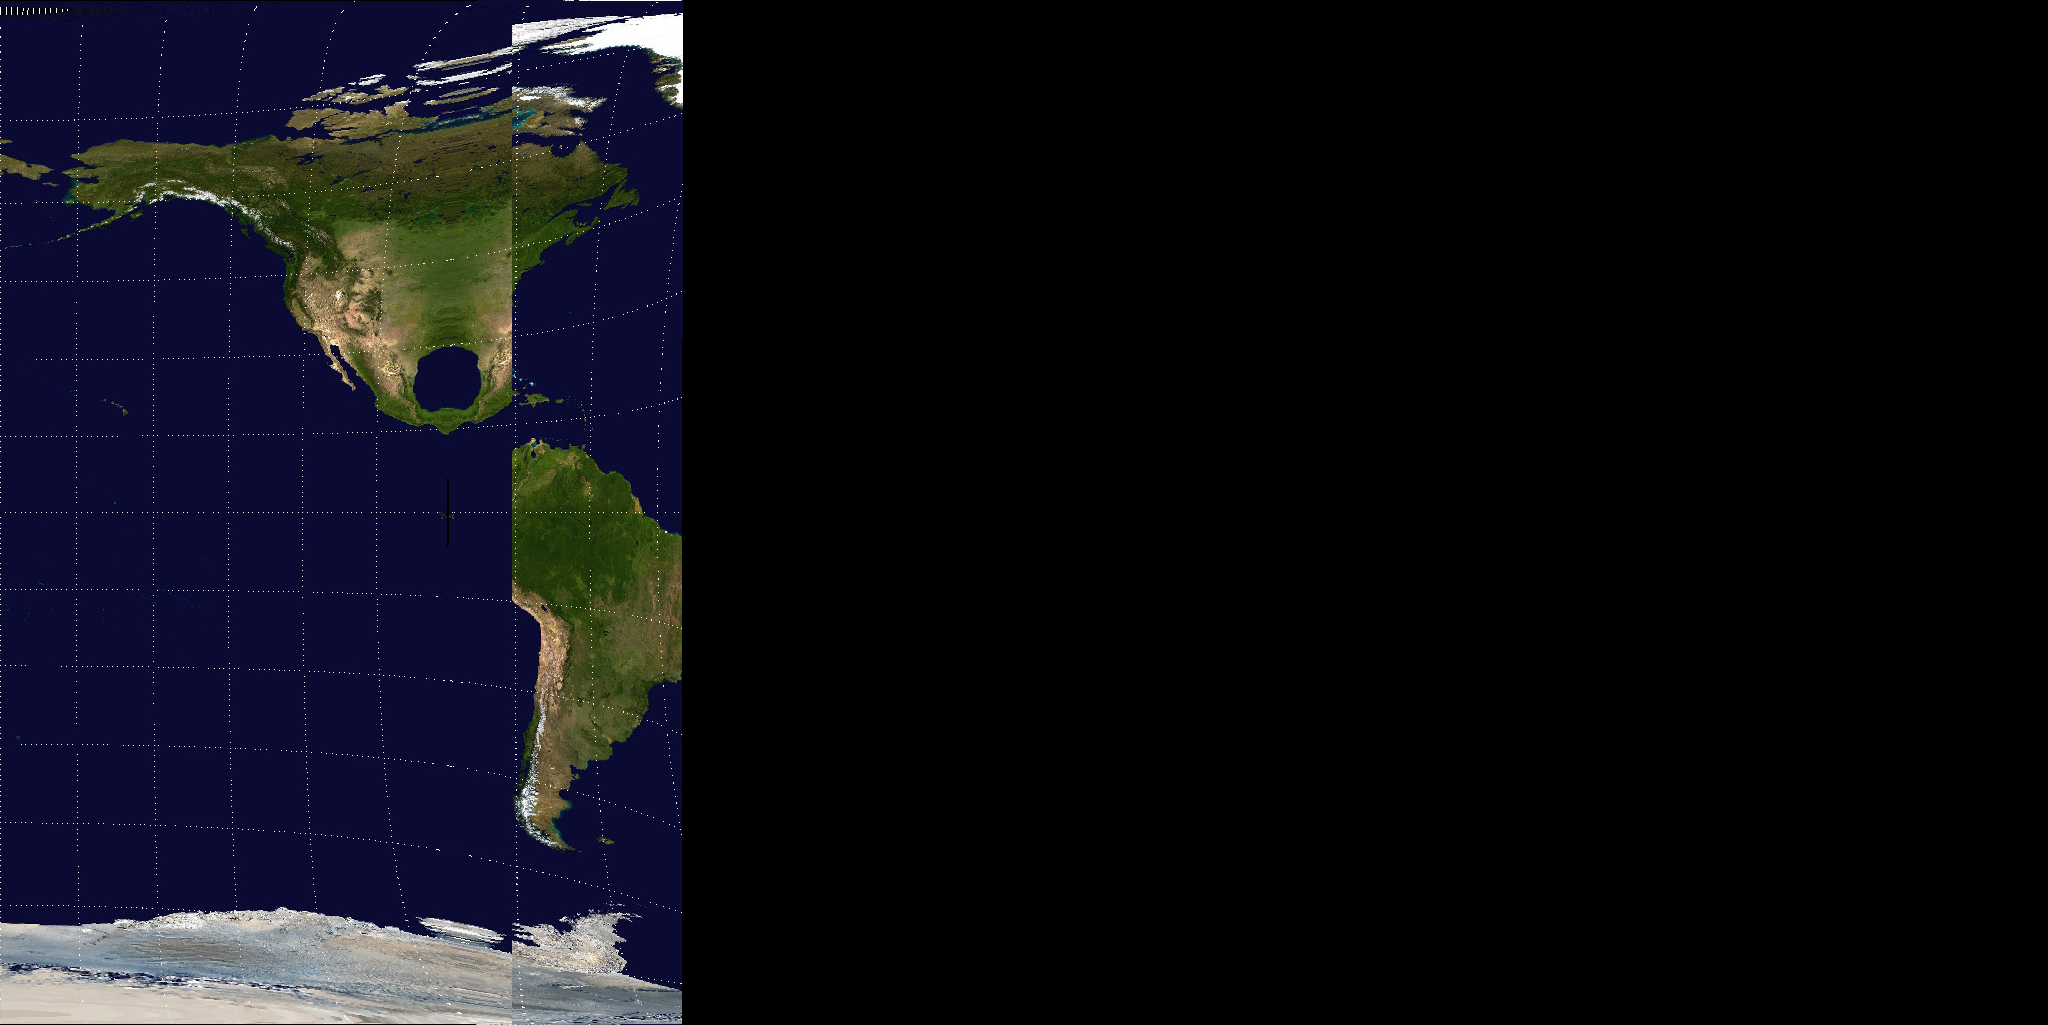
\includegraphics[width=.35\textwidth]{output_onethird}};
    \node (out2) at (\hoffset,0pt)
      {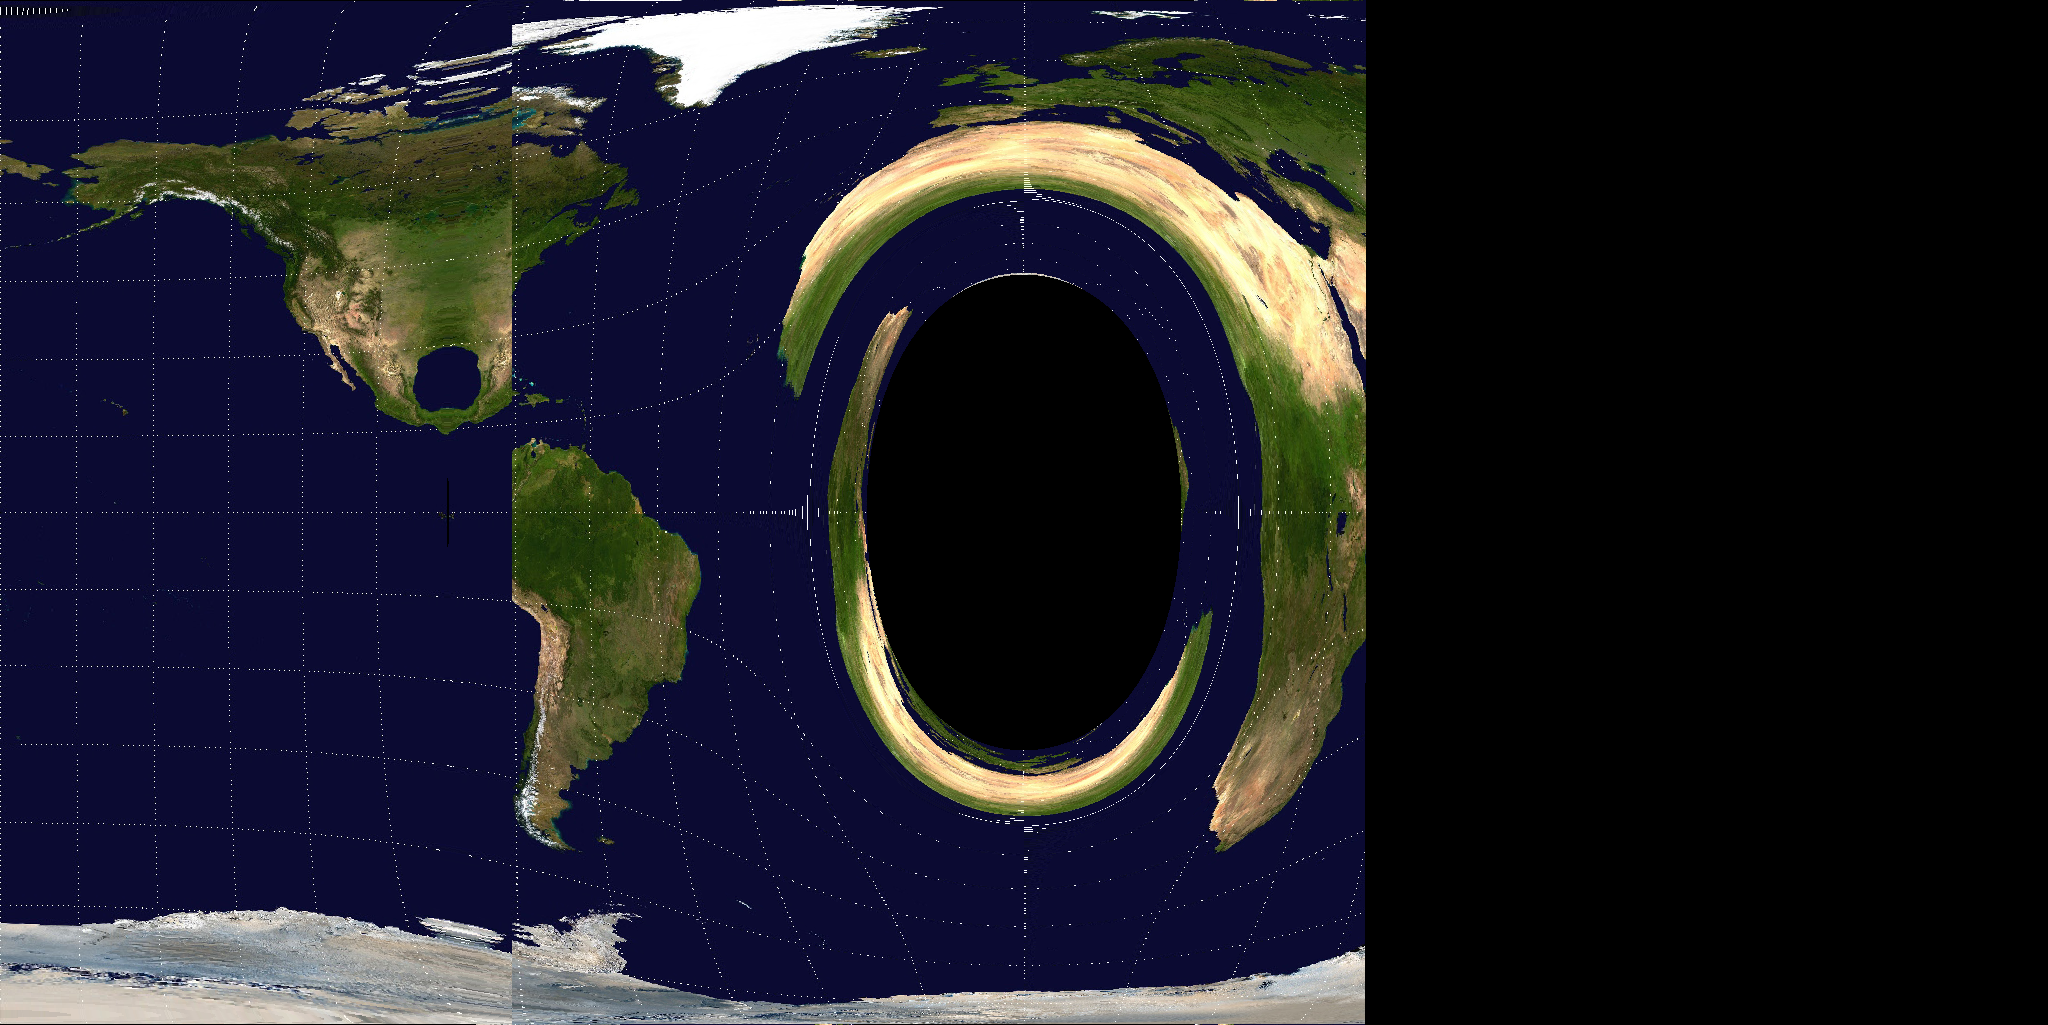
\includegraphics[width=.35\textwidth]{output_twothird}};
    \node (out3) at (\hoffset,-\voffset)
      {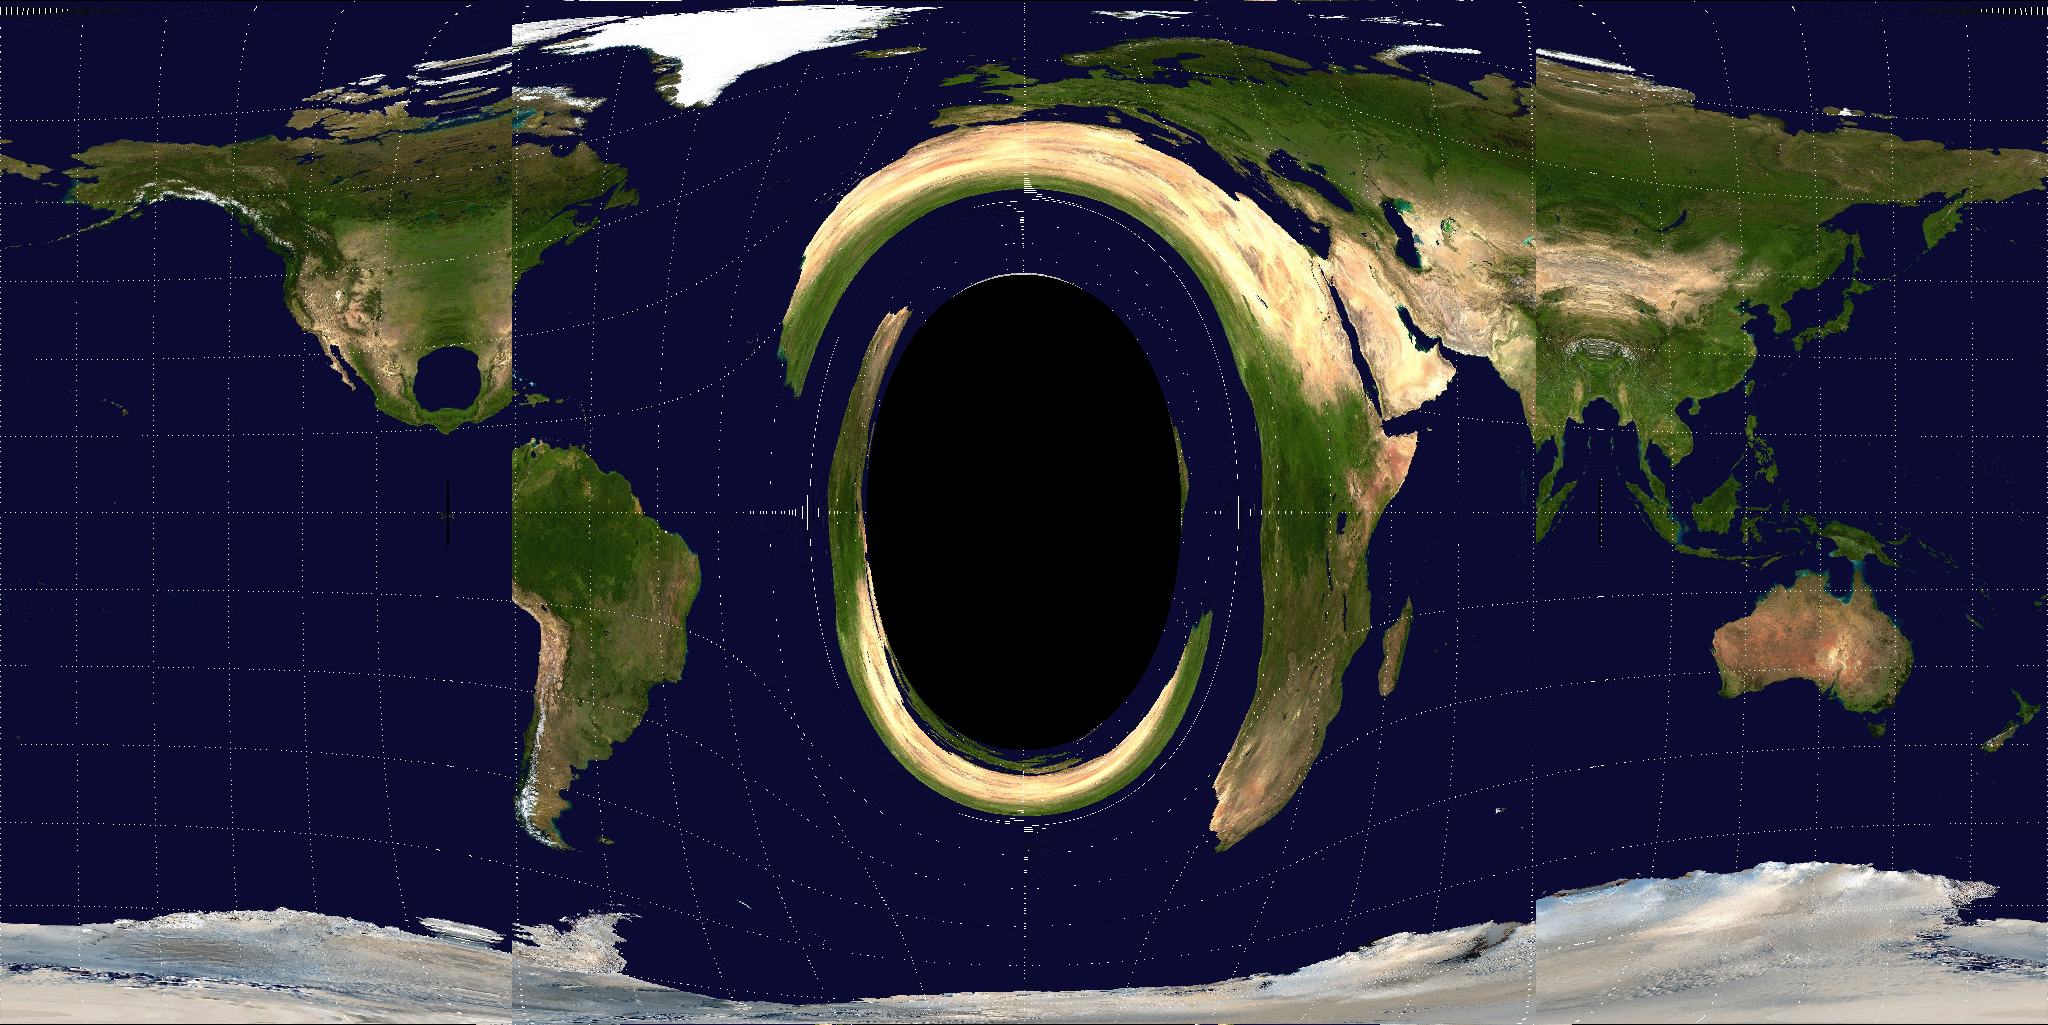
\includegraphics[width=.35\textwidth]{output_full}};
    \draw[->,shorten <=5mm,shorten >=5mm] (in) -- (out2);
    \draw[->] (out1) -- (out2);
    \draw[->] (out2) -- (out3);
  \end{tikzpicture}
\end{figure*}

\end{document}


\section{Results}
\documentclass{standalone}

\begin{document}
\begin{figure*}
  \caption{\label{fig:earthsample}
    Sample image used to test the application of a generated lensing map.
  }
  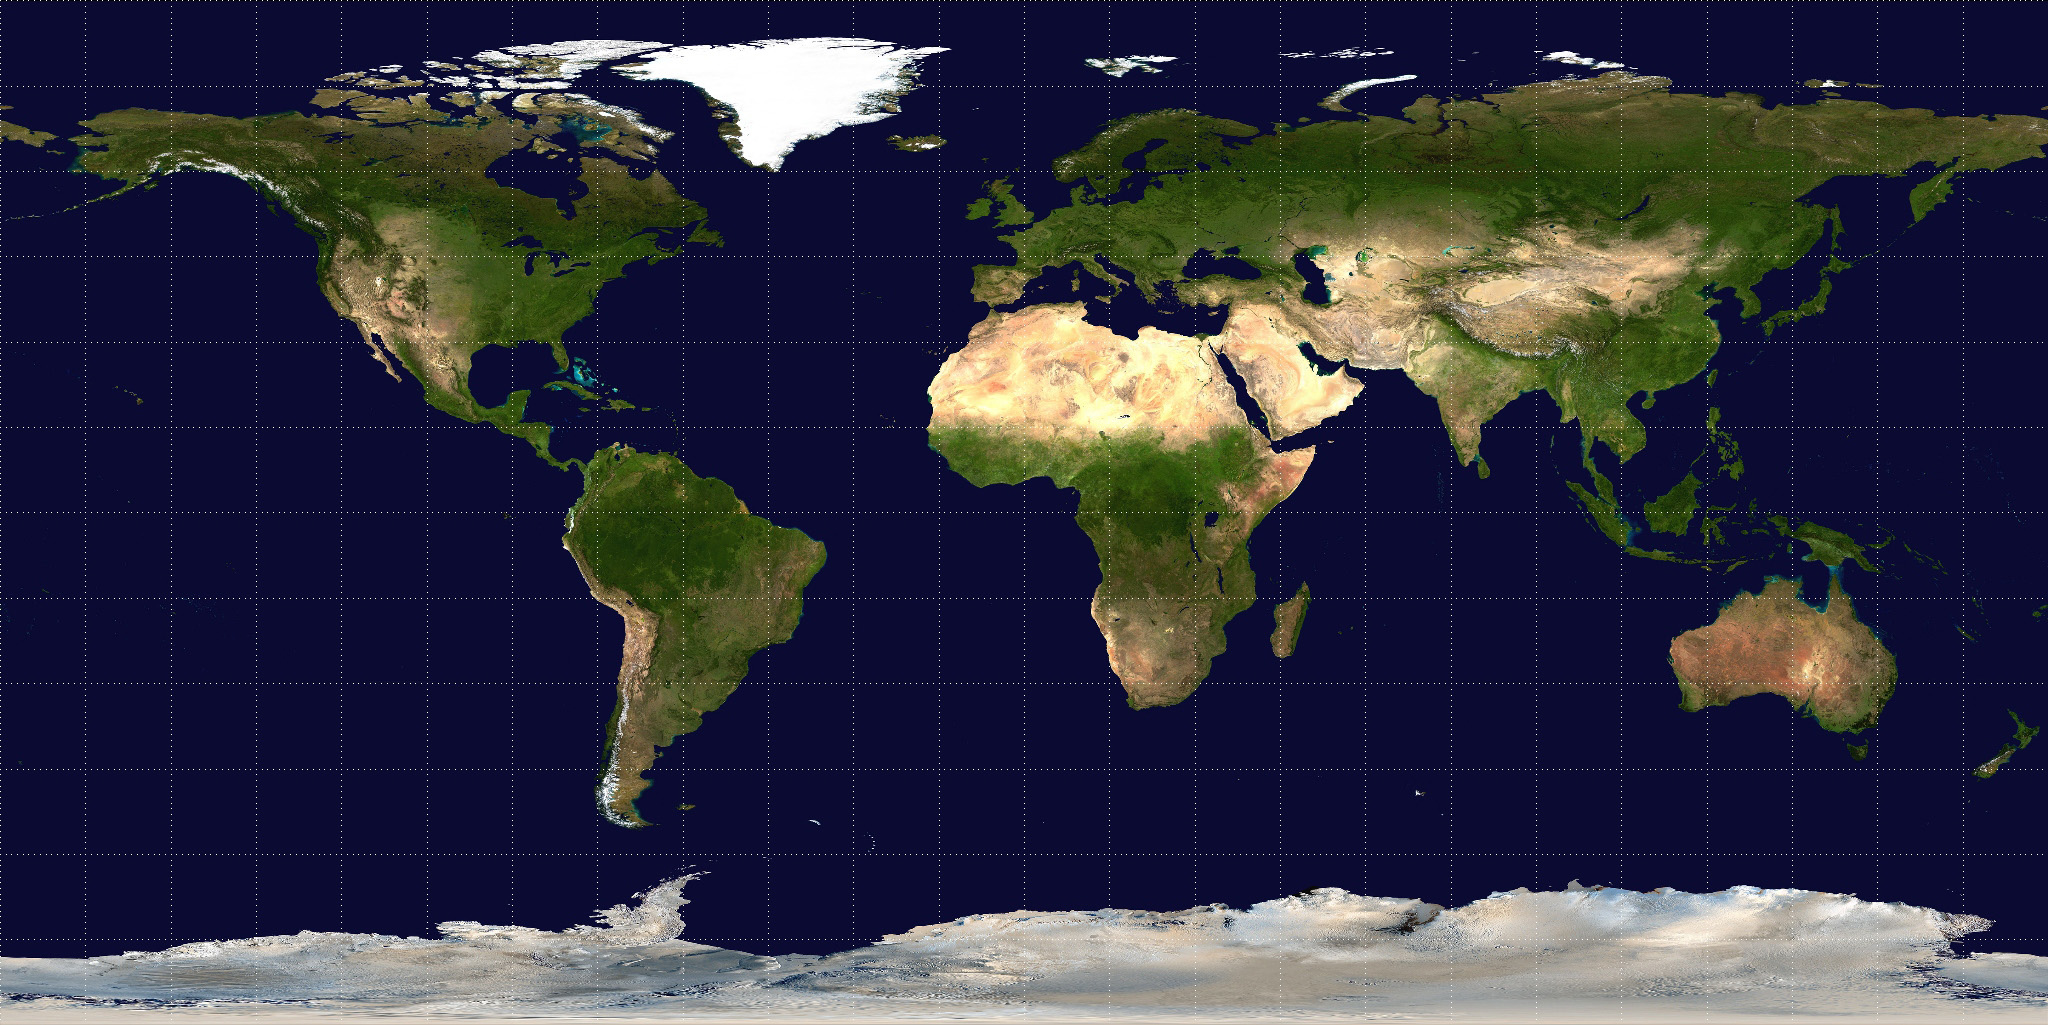
\includegraphics[width=\textwidth]{earth}
\end{figure*}

\begin{figure*}
  \caption{\label{fig:example1}
    Final result of applying the explicit Schwarzschild lensing map on the sample image shown in Fig.(\ref{fig:earthsample}) using a Schwarzschild space-time defined by $M=\SI{1}{\kilo\meter}$ and $R_O=\SI{10}{\kilo\meter}$.
    In this example, one can easily see the problematic image tearing at the $\pi/2$ and $-\pi/2$ meridians.
  }
  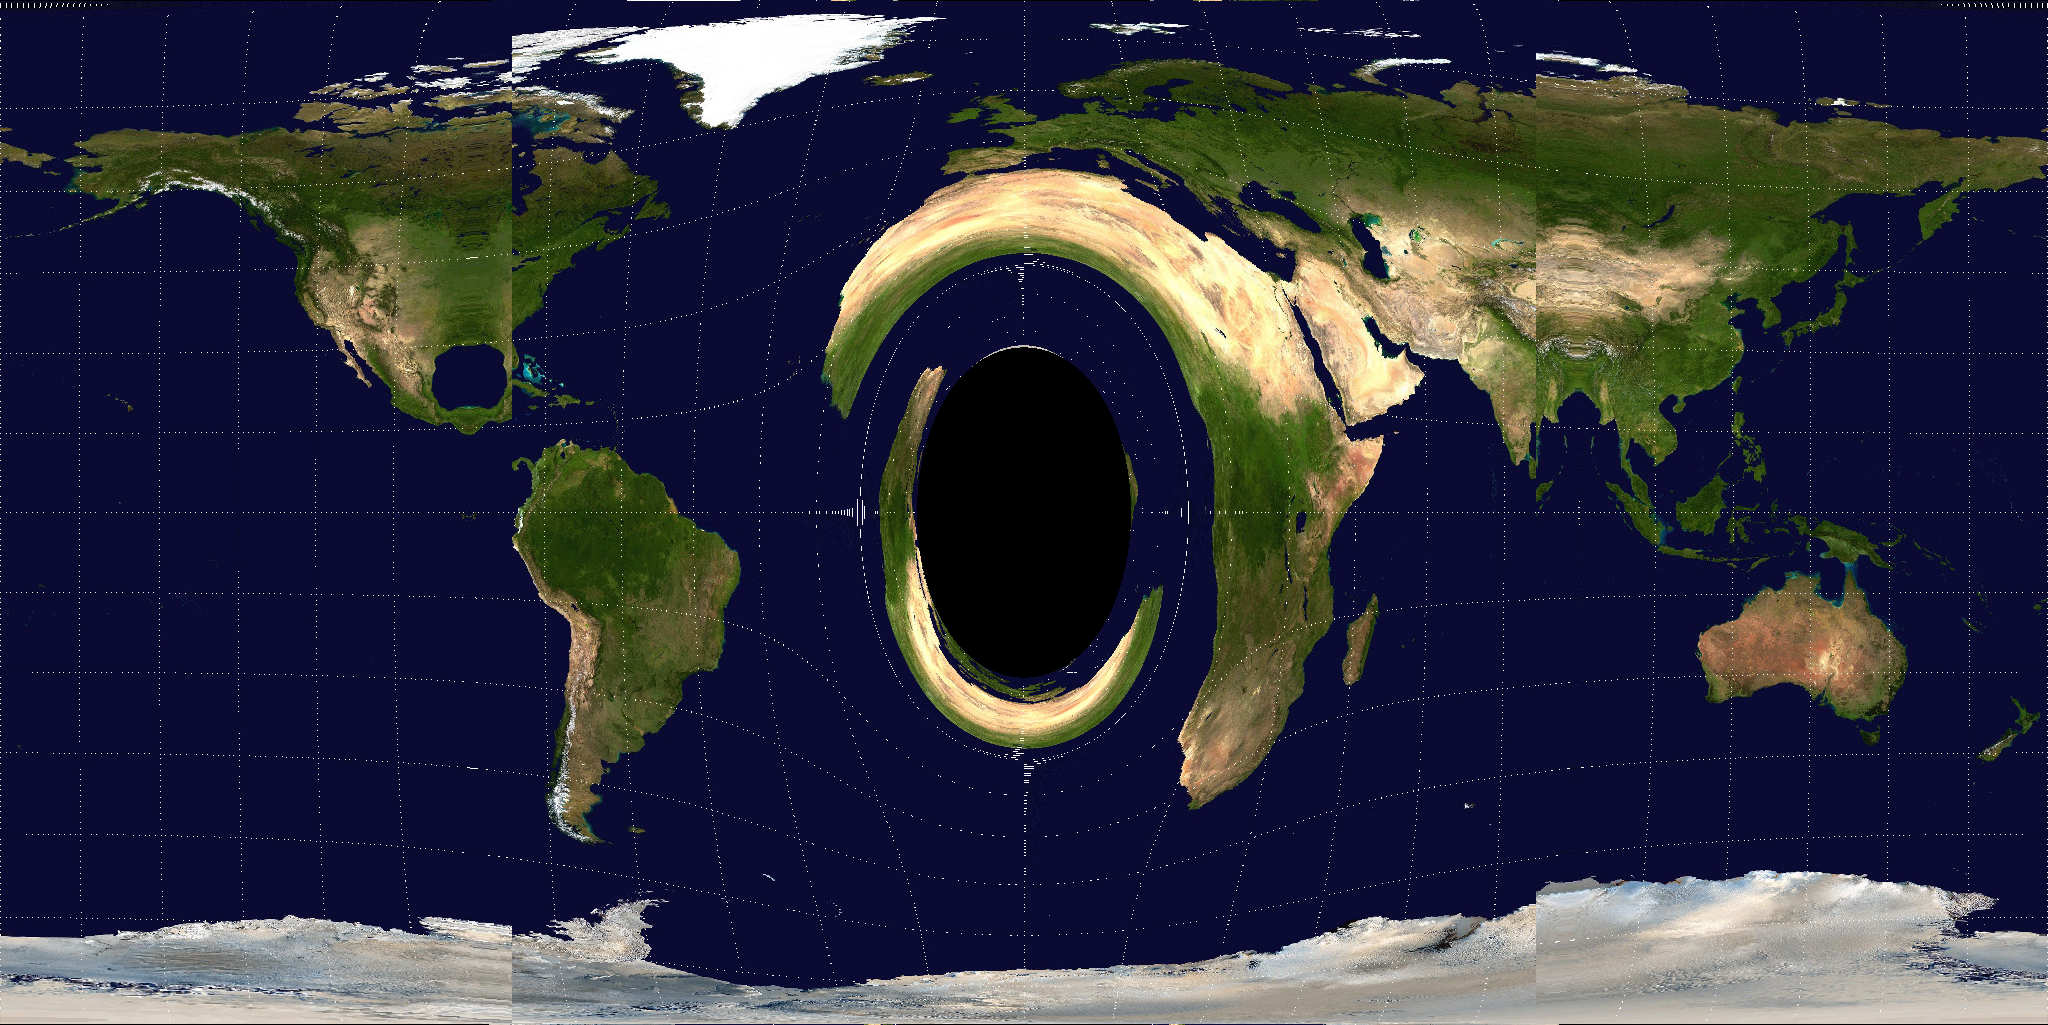
\includegraphics[width=\textwidth]{example_lens1}
\end{figure*}

\begin{figure*}
  \caption{\label{fig:example2}
    Second example of a generated Schwarzschild lensing map using the same space-time as in Fig.(\ref{fig:example1}) but at a radius of $R_O=\SI{2.5}{\kilo\meter}$, which is significantly closer to the event horizon.
    The accuracy of this result hasn't yet been scrutinized, however the overall converging of the observer's sky to the point at $\phi=0$ is to be expected.
  }
  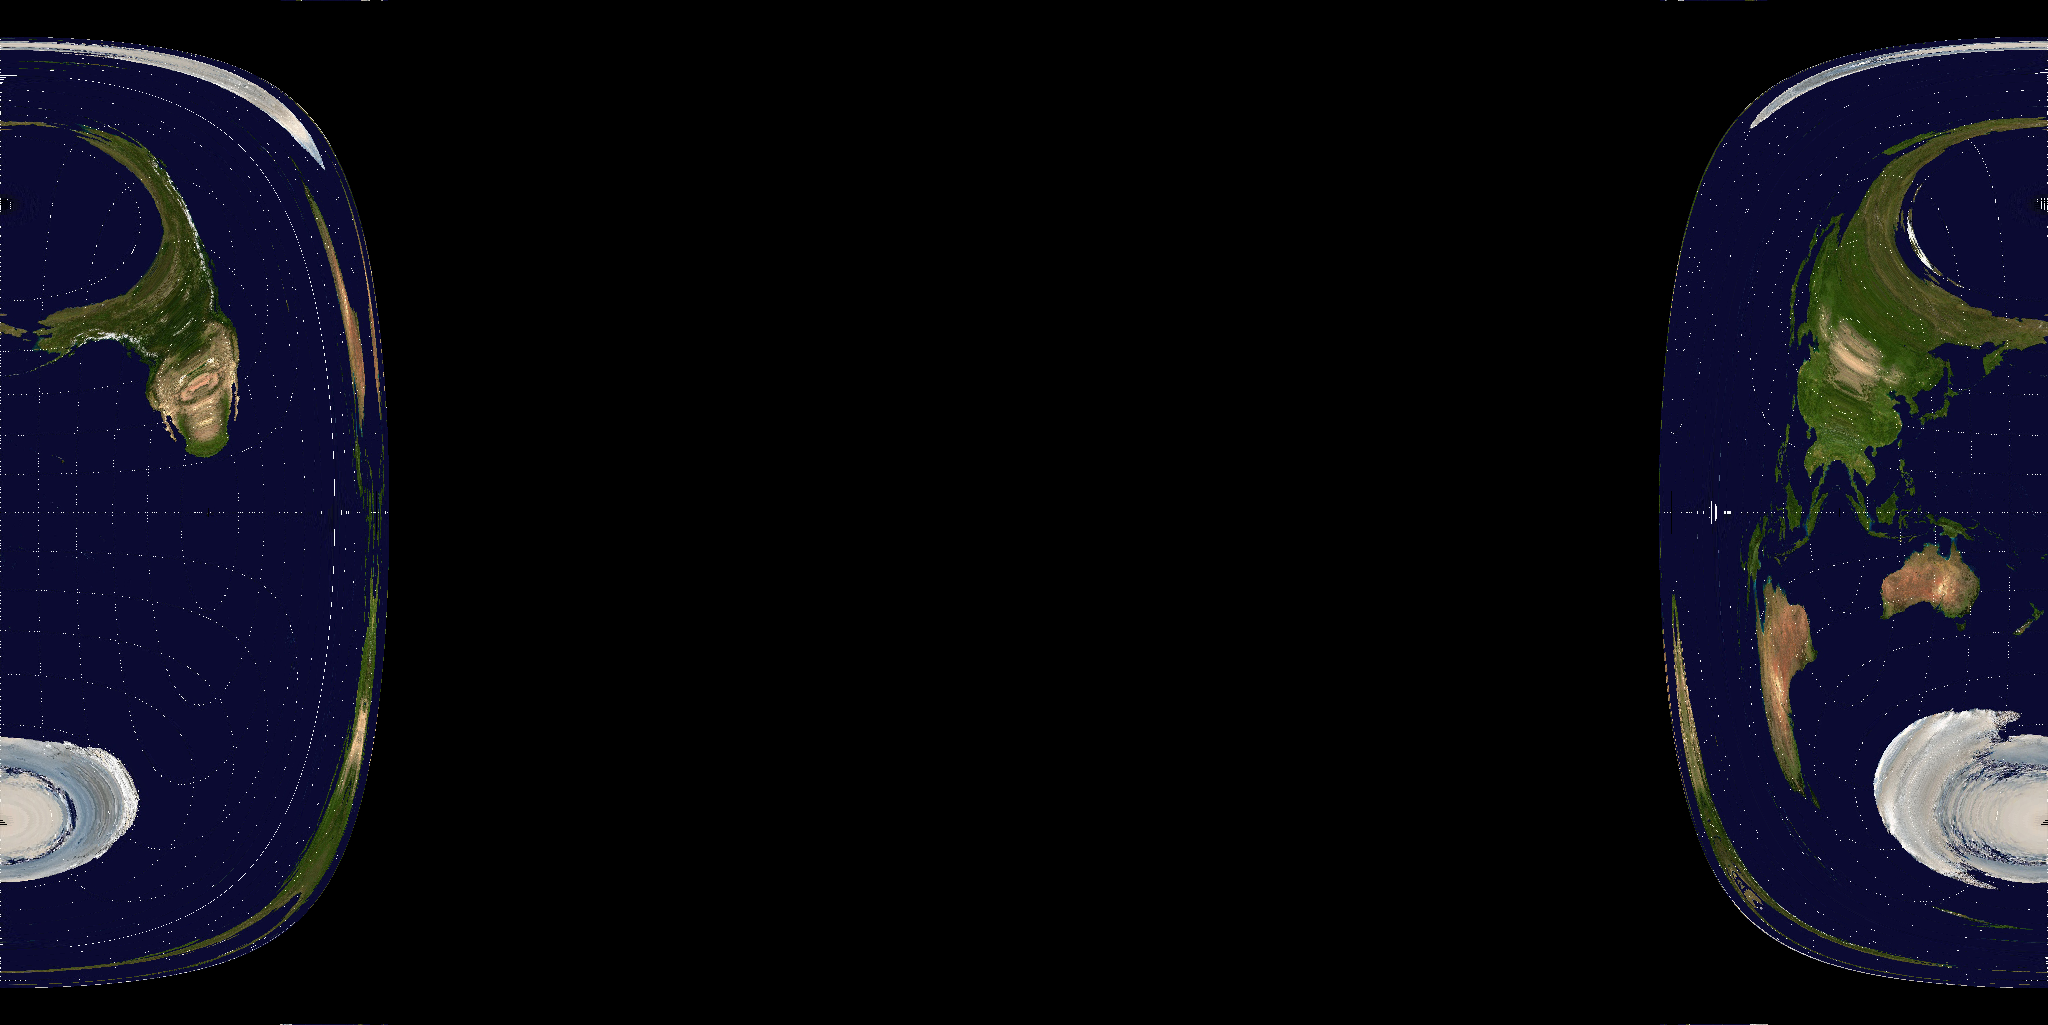
\includegraphics[width=\textwidth]{example_lens2}
\end{figure*}

\begin{figure*}
  \caption{\label{fig:lenscomparison}
    Comparison between the three levels of approximation in the Schwarzschild lensing equation.
    The first graph indicates the differences near the singularity, while the latter shows that the amount of error decreases significantly as the radius of the observer increases.
  }
  \begin{tabular}{c}
    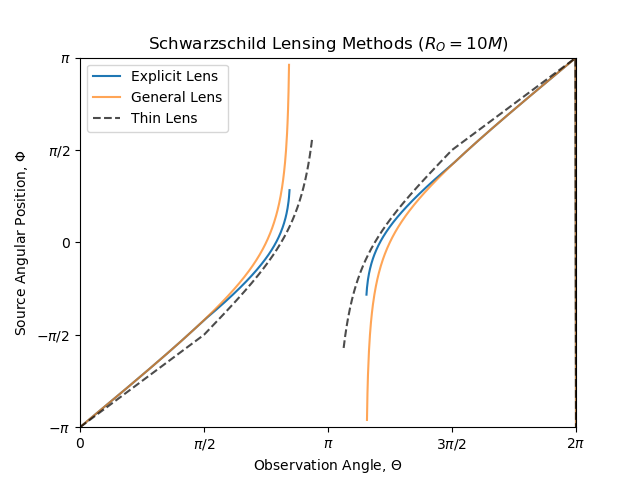
\includegraphics[width=.75\textwidth]{sc_lensing_near}\\
    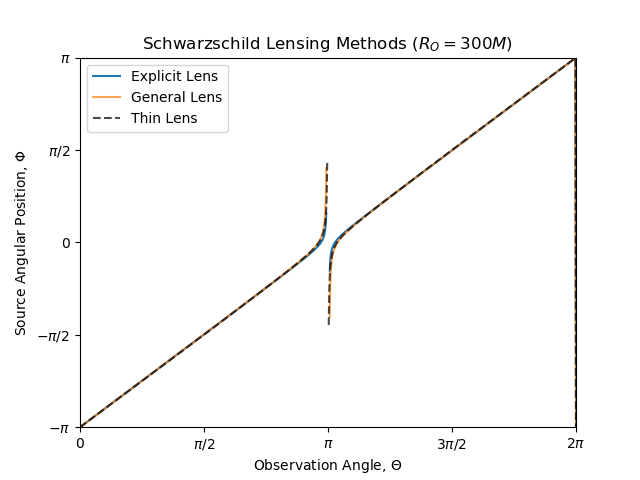
\includegraphics[width=.75\textwidth]{sc_lensing_far}
  \end{tabular}
\end{figure*}

\end{document}


\section{Discussion and Conclusion}
\documentclass{standalone}

\begin{document}


\end{document}


\end{document}
